%! TEX program = xelatex
\documentclass{report}
% provides basic settings for ctex document
\usepackage[UTF8, heading=true]{ctex}
\usepackage{fancyhdr}
\usepackage{tocloft}
\usepackage[margin=1in]{geometry}
\usepackage{metalogo}                   % \XeLaTeX
\usepackage{float}                      % figure H flag
\usepackage{microtype}                  % break long words
\usepackage[hidelinks]{hyperref}
\usepackage{tabularx}
\usepackage{amsmath}
\usepackage{lmodern}                    % allow fonts to scale
\usepackage{placeins}
\usepackage{multirow}                   % multirow, multicolumn support
\usepackage{booktabs}                   % toprule, cmidrule support
\usepackage{caption}

% make chapter stay in the same page
%\makeatletter
%\renewcommand\chapter{\thispagestyle{plain}%
%\global\@topnum\z@
%\@afterindentfalse
%\secdef\@chapter\@schapter}
%\makeatother

\fancyhead{}
\renewcommand{\sectionmark}[1]{\markleft{#1}}
\renewcommand{\partmark}[1]{\markright{#1}}
\lhead{\tiny \leftmark}
\rhead{\tiny \rightmark}
% see $(texdoc ctex) for details
\ctexset{
    chapter = {
        name = {实验},
        format += \flushleft,
        number = \arabic{chapter},
    },
    section = {
        format += \flushleft,
    },
    appendix = {
        number = \Alph{chapter},
        name = {附录},
    },
}

\pagestyle{fancy}
%\setlength\cftaftertoctitleskip{2em}

% provides code input support
\usepackage{xparse}                     % newcommand multiple optional arguments
\usepackage{listings}                   % code
\usepackage{fontspec}
\usepackage{lmodern}

%\newfontfamily\codeF{Fira Code}

\setmonofont[
    Contextuals={Alternate},
    ItalicFont = Fira Code      % to avoid font warning
]{Fira Code}

% usage: \inputCode{[language] <path>}
% if language is not explicitly set, it's defaulted to c
\DeclareDocumentCommand{\inputCode}{ O{c} m }{
    {
        \lstinputlisting[
            basicstyle=\small\ttfamily,
            language={#1},
            tabsize=4,
            showstringspaces=false,
            breaklines=true,
            frame=shadowbox,
            framexleftmargin=10mm,
            rulesepcolor=\color{black},
            numbers=left,
            xleftmargin=4em,
        ]{#2}
    }
}

\DeclareDocumentCommand{\inputCodeSetLanguage}{ m }{
    \lstset{
        basicstyle=\small\ttfamily,
        language={#1},
        tabsize=4,
        showstringspaces=false,
        breaklines=true,
        frame=shadowbox,
        framexleftmargin=10mm,
        rulesepcolor=\color{black},
        numbers=left,
        xleftmargin=4em,
    }
}

\DeclareDocumentCommand{\inputCodeNoNumberSetLanguage}{ m }{
    \lstset{
        basicstyle=\small\ttfamily,
        language={#1},
        tabsize=4,
        showstringspaces=false,
        breaklines=true,
        frame=shadowbox,
        rulesepcolor=\color{black},
    }
}


\usepackage{xparse}
\usepackage{tcolorbox}
\usepackage{mdframed}

\tcbuselibrary{breakable}
\NewDocumentCommand{\exercise}{ m +m }{
    {
        \edef\originalParIndent{\the\parindent}
        \begin{tcolorbox}[breakable,arc=0mm,boxrule=0.4pt]
            \setlength{\parindent}{\originalParIndent}
            \noindent
            \textbf{\large Exercise #1}
            \indent
            #2
        \end{tcolorbox}
    }
}

% environment style of exercise, to feed special requirements
\NewDocumentEnvironment{exerciseEnv}{m}{
    \edef\originalParIndent{\the\parindent}
    \begin{tcolorbox}[breakable,arc=0mm,boxrule=0.4pt]
        \setlength{\parindent}{\originalParIndent}
        \noindent
        \textbf{\large Exercise #1}
        \indent
} {
    \end{tcolorbox}
}

\NewDocumentEnvironment{questionEnv}{}{
    \edef\originalParIndent{\the\parindent}
    \begin{tcolorbox}[breakable,arc=0mm,boxrule=0.4pt]
        \setlength{\parindent}{\originalParIndent}
        \noindent
        \textbf{\large Question}
        \indent
} {
    \end{tcolorbox}
}

% a raised rule
\NewDocumentCommand{\raisedrule}{ O{0em} m }{\leaders\hbox{\rule[#1]{1pt}{#2}}\hfill}

\NewDocumentEnvironment{exerciseSolution}{m}{
    {\noindent \textbf{\large Exercise #1 实验过程 \raisedrule[0.3em]{0.6pt}}}
} {
    \par
    {\noindent \textbf{\large \raisedrule[0.3em]{0.6pt} Exercise #1 实验过程}}
    \vspace{1em}
}

\NewDocumentEnvironment{answer}{}{
    {\noindent \textbf{\large Answer \raisedrule[0.3em]{0.6pt}}}
} {
    \par
    {\noindent \textbf{\large \raisedrule[0.3em]{0.6pt} Answer}}
    \vspace{1em}
}



%%%%%%%%%%%%%%%%%%%%%%%%%%%%%%%%
\graphicspath{{./res/}}

%%%%%%%%%%%%%%%%%%%%%%%%%%%%%%%%
% Code Area Define
\usepackage{listings}
\usepackage{color}

\definecolor{dkgreen}{rgb}{0,0.6,0}
\definecolor{gray}{rgb}{0.5,0.5,0.5}
\definecolor{mauve}{rgb}{0.58,0,0.82}

\lstset{frame=tb,
  language=C++,
  aboveskip=3mm,
  belowskip=3mm,
  showstringspaces=false,
  columns=flexible,
  basicstyle={\small\ttfamily},
  numbers=none,
  numberstyle=\tiny\color{gray},
  keywordstyle=\color{blue},
  commentstyle=\color{dkgreen},
  stringstyle=\color{mauve},
  breaklines=true,
  breakatwhitespace=true,
  tabsize=3
}
%%%%%%%%%%%%%%%%%%%%%%%%%%%%%

% report content %%%%%%%%%%%%
%%%%%%%%%%%%%%%%%%%%%%%%%%%%%
\begin{document}

% cover page
\begin{titlepage}
    \addtolength{\topmargin}{1cm}
    \centering
    
\includegraphics[width=0.6\textwidth]{hust.jpg}\par
    \vspace{0.5cm}
    {\Huge \heiti 嵌入式实验报告}\par
    \vspace{10cm}
    {
        \large
        \begin{tabular}{r m{8em}}
            \makebox[6em][s]{学生姓名}:& 刘本嵩 \\ \cline{2-2}
            \makebox[6em][s]{学号}:& U201614531\\ \cline{2-2}
            %\makebox[6em][s]{学生姓名}:& 潘璐 \\ \cline{2-2}
            %\makebox[6em][s]{学号}:& U201614539\\ \cline{2-2}
            \makebox[6em][s]{专业}:& 计算机科学与技术\\ \cline{2-2}
            \makebox[6em][s]{班级}:& CS1601\\ \cline{2-2}
            \makebox[6em][s]{指导教师}:& 张杰 \\ \cline{2-2}
        \end{tabular}
    }
    \vfill
    \today
\end{titlepage}

\setcounter{tocdepth}{1}
\pagenumbering{Roman}
\tableofcontents

\newpage
\pagenumbering{arabic}
\setcounter{page}{1}



\chapter{核心编译,系统烧录}
\section{实验内容}

\begin{enumerate}
    \item 系统镜像的编译生成
        \begin{itemize}
            \item Uboot编译(不要求)
            \item Kernel编译
            \item Android系统编译(不要求)
        \end{itemize}
    \item Android+Linux系统烧录
        \begin{itemize}
            \item 串口工具cutecom使用,控制uboot
            \item usb烧写工具fastboot使用
        \end{itemize}
    \item 简单Linux应用程序开发
        \begin{itemize}
            \item 使用Android NDK编译简单应用程序
            \item 使用usb开发工具adb上传并运行程序
        \end{itemize}
\end{enumerate}

\section{实验设计}
\par 首先熟悉Linux Kernel目录结构
\begin{itemize}
    \item arch:与体系结构有关的代码,zimage在arch/arm/boot下;
    \item drivers:包括所有的驱动程序
    \item fs:各种文件系统格式支持源码;
    \item ipc:System V的进程通信实现,包括信号量,共享内存;
    \item kernel:进程调度,创建,定时器,信号处理等;
    \item mm:内存管理;
    \item net:套接字和网络协议的实现;
\end{itemize}
\par 然后使用make menucongif命令,图像化配置内核。接着在核心源代码根目录下执行make zImage命令生成内核镜像zImage。然后开始系统烧写的准备工作。在用户根目录下编辑adb\_usb.ini文件。若没有该文件,创建一个。接着进行设备的连接工作。

\section{实验过程}
\par 首先修改common/rules.mk,增加便于使用的规则burn,同时修改使用更好的编译选项。下面仅列出
修改部分,且在下文不再重复。

\begin{lstlisting}
CFLAGS:=--sysroot=$(DIR)/platforms/android-9/arch-arm -march=armv7-a -mfloat-abi=softfp -mfpu=neon -O1 -Wall -Wextra -std=c99
burn: clean $(EXENAME)
	adb push $(EXENAME) /data/local/$(EXENAME) && adb shell /data/local/$(EXENAME)
\end{lstlisting}


\begin{enumerate}
    \item 为ARM编译安装Linux内核。
        \begin{itemize}
            \item make xconfig \# 我喜欢xconfig
            \item make zImage
            \item 连接好设备,打开cutecom,按要求进入fastboot模式,下面开始写系统。
            \item sudo fish
            \item fastboot flash kernel zImage \# 已经在root,且系统已经安装fastboot。无需从目录启动旧版。
            \item fastboot flash ramdisk ramdisk-uboot.img
            \item fastboot -w
            \item fastboot flash system system.img
            \item 下面使用cutecom输入bootargs指令。
            \item setenv bootcmd movi read kernel 0 40008000;movi read rootfs 0 41000000 100000;bootm 40008000 41000000
            \item setenv bootargs
            \item saveenv
        \end{itemize}
    \item 编译生成lab1:
        \begin{itemize}
            \item make
        \end{itemize}
    \item 把文件上传到实验板上的/data目录并运行:
        \begin{itemize}
            \item make burn
        \end{itemize}
\end{enumerate}

\chapter{Linux framebuffer界面显示开发}
\section{实验内容}
\begin{enumerate}
    \item Linux下的LCD显示驱动接口:framebuffer的使用原理。
    \item 基本图形的显示:点、线、矩阵区域。
    \item 双缓冲机制
\end{enumerate}

\section{实验设计}
\par 首先了解Linux framebuffer驱动原理。
\begin{itemize}
    \item 通过framebuffer,应用程序用mmap把显存映射到程序虚拟地址空间,将要显示的数据写入写个内存空间就可以在屏幕上显示出来。
    \item 驱动程序分配系统内存作为显存;实现file\_operation结构中的接口,为应用程序服务;实现fb\_ops结构中的接口,控制和操作LCD控制器。
    \item 驱动程序将显存的起始地址和长度传给LCD控制器的寄存器(一般由fb\_set\_var完成),LCD控制器会自动的将显存中的数据显示在LCD屏幕上。
\end{itemize}

\par 实验中需要使用的双缓冲机制如下:
\par 一般情况下,最终的用户界面都需要经过若干次绘图才能完成,比如要先擦除之前的界面内容,再绘制新的界面内容,如果这些中间绘图是直接在framebuffer上操作,那么在LCD屏幕上就会看到这些中间结果。比如会看到屏幕先被清除,再显示出来界面,而不是界面内容直接出现在屏幕上。这就是屏幕闪烁。解决屏幕闪烁的办法就是双缓冲,所有的绘图都先绘制在一个后缓冲中(后缓冲:和framebuffer同样大小的一块内存)。绘制完毕后再把最终屏幕内容拷贝到framebuffer中。

\par 双缓冲的绘图过程:

\begin{itemize}
    \item 所有的绘图函数都在后缓冲中绘图。
    \item 所有的绘图函数都要记录本次的绘图区域:void \_update\_area(int x, int y, int w, int h)
    \item 绘图完毕后,把后缓冲中所有需要更新的绘图区域内容拷贝到前缓冲: void fb\_update(void);
    \item 清空需要更新的绘图区域;
\end{itemize}

\par 双缓冲机制的扩展:
\begin{itemize}
    \item 前后缓冲可以交换:前缓冲内存内容对应屏幕的显示,前缓冲内存的首地址是可以修改的(显卡驱动支持,一个寄存器的内容) 后缓冲绘制完之后,交换前后缓冲
    \item 帧同步信号(垂直同步信号 VSYNC): 硬件DMA周期性(60Hz)的扫描读取前缓冲的内存,传递 给LCD控制器显示。每次完整传输完一帧图像都有一个帧同 步信号,然后等待大约16ms之后再重新开始。
\end{itemize}

\section{实验过程}
\subsection{通用优化}
\par 首先,每个画点函数都调用update将会浪费大量CPU时间。我实现了一个raw\_draw\_pixel,在其他绘画函数中调用它,而不是重新检查边界。这将大大加快运行速度。
\par 其次,main中过快的刷新率使得CPU为人眼根本无法看清的细节浪费了大量CPU时间。我调整了fb\_update,减慢了不必要的刷新,使得画点、画线、画矩形都能在人眼无法分辨的情形下将时间缩短到2毫秒内。(被要求移除此优化)
\par 其次,上一节中在编译选项中加入-O3和-std=c99,不但速度加快,还发现了库中的若干软件错误。下一次实验将会详细描述这些错误。

\subsection{画线函数}
\par 画线函数的大致思路为:首先计算所划线的斜率的绝对值,若斜率的绝对值大于一,则交换x1和y1的值,x2和y2的值。画线的时候对于所画线的斜率分为两种情况,斜率绝对值大于1的情况和斜率绝对值小于一的情况。具体的实现就是按照计算得出的斜率值,每次画出一个点以后,就使用斜率值计算出下一个点的位置,然后调用画点函数进行画点,直到画出所有的点。
%avoid being fucked.%\begin{figure}[htpb]
%avoid being fucked.%    \centering
%avoid being fucked.%    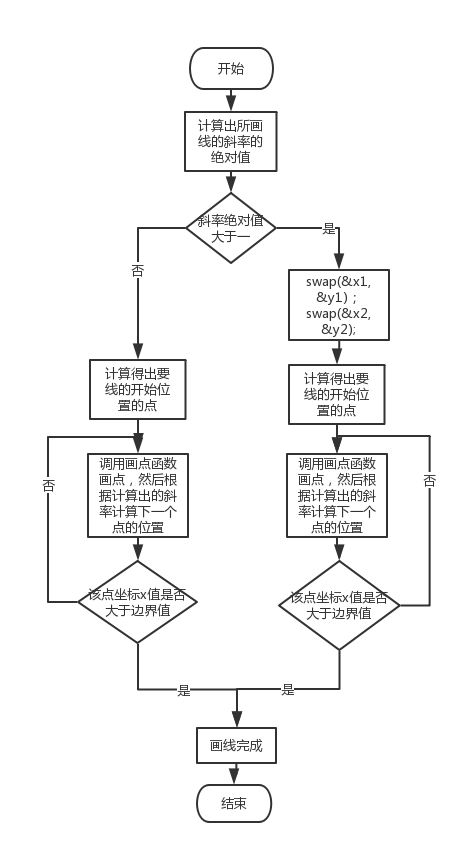
\includegraphics[width=0.35\linewidth]{drawline.png}
%avoid being fucked.%    \caption{画线函数流程}
%avoid being fucked.%    \label{fig:drawline}
%avoid being fucked.%\end{figure}

\subsection{画矩形函数}
\par 矩形函数的主要思路为:首先检查输入的坐标是否越界,然后调用update函数,使用两个for循环绘制所有点即可。

\chapter{图片显示和文本显示}
\section{实验内容}

\begin{enumerate}
    \item JPEG不透明图片显示
    \item PNG半透明图片显示
    \item 矢量字体显示:
        \begin{enumerate}
            \item 字模的提取
            \item 字模的显示(只有alpha值的位图)
        \end{enumerate}
\end{enumerate}

\section{实验设计}

\par 同实验二相似,实验三也需要我们直接操作FrameBuffer将屏幕上每一个像素点的RGB值更新。
\par 实验框架已经提供了相应的图片、字体解析接口将图片和字体转换成统一的、可以被直接解析的格式;实验框架也提供了基于现实字体封装的显示字符串的函数。
\par 在实验三中,我们无需关注图片、字体格式的细节(图片编码、字模),只需处理调用相应接口后返回的\lstinline|fb_image|即可。
\par 需要注意的是,PNG图片和字体需要能支持Alpha通道(即透明度通道),透明度叠加的公式实验讲义已经给出。

\section{实验过程}
\subsection{JPEG图片显示}
\par JPEG的图片无需计算透明度,而且其格式与FrameBuffer的格式相似,可以直接采用单循环按行进行内存拷贝。该实现缓存友好、效率较高。 显示JPEG图片的流程如图\ref{fig:jpeg}所示。

\subsection{PNG图片显示}
\par PNG图片由于涉及透明度,所以显示时采用的方式是依次遍历待显示每一个像素点,根据像素点的Alpha值以及对应FrameBuffer的三通道(R、G、B)值分别新的通道值并写入FrameBuffer。
\par 当Alpha值为0或是255时,无需考虑Alpha值以及相关的计算,以节省计算资源。
\par 实际上,可以把每一个M*N图片转换成三个M*N的颜色矩阵——R矩阵、G矩阵、B矩阵。所有的透明度计算均可以变为矩阵的相关运算。这样可以充分利用缓存的特性、同时优化运算。出于时间和难度等原因,未采用这种实现。
\par 有其他同学提到,在实现时遇到了程序SegmentFault的错误,并且确定了原因是:

\begin{enumerate}
    \item 未对边界进行合理的检查,导致出现了超过FrameBuffer的地址的写入。
    \item 程序开启了-O3编译优化参数,部分激进的优化使得程序出错。
\end{enumerate}
\par \strong{其实这种调查结论只是权宜之计。}我也开启了-O3,同时开启了c99标准发现了以下致命错误:

\begin{enumerate}
    \item common/external.c没有include time.h
    \item common/external.c:fb\_new\_image函数有两处本该返回NULL或image,却漏写返回值。C89以神奇的容错性允许了这种写法。
    \item common/external.c:fb\_get\_sub\_image函数的i应当是unsigned int。
    \item 其他非致命问题。
\end{enumerate}

只需修复这些错误,程序的行为自然恢复可控。实验中明明使用了虽然落后但支持c99的gcc4编译器,大家却都在使用
老旧的c89标准,它甚至不会发出warning,以至于无人发现第二条的致命错误。

%\par 显示PNG图片的流程如图\ref{fig:png}所示。
%\begin{figure}[htpb]
%    \centering
%    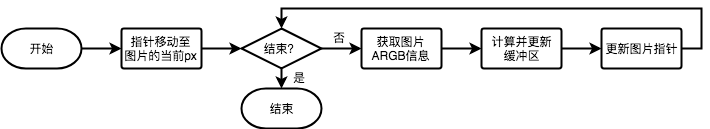
\includegraphics[width=0.8\linewidth]{png.png}
%    \caption{Png显示图片流程}
%    \label{fig:png}
%\end{figure}

\subsection{字体显示}
\par 字体显示同PNG显示几乎一样。但是在实现时遇到了字体宽度只有原字体宽度1/4的情况。这是因为字体图片和PNG图片的格式不同。字体图片中的每一个字节只代表Alpha值,而R、G、B值由函数入口参数color提供。因此还需要对字体显示的部分代码进行修改,补齐缺少的R、G、B三通道颜色的计算。修改完成后,实验结果正确。

\chapter{Linux touchscreen多点触摸开发}
\section{实验内容}
\begin{enumerate}
    \item Linux下的触摸屏驱动接口:
        \begin{enumerate}
            \item Input event的使用
            \item 多点触摸协议(Multi-touch Protocol)
        \end{enumerate}
    \item 获取多点触摸的坐标
    \item 在LCD上显示多点触摸轨迹
    \item 绘制一个清除屏幕的按钮,点击后清除屏幕内容
\end{enumerate}
\section{实验设计}
\par Linux下的触摸屏驱动接口以及实验相关的框架代码已经给出。设备驱动的初始化也已经提供。其本质是一个忙等待的无限循环,在循环内部,程序主动地调用相关函数,获取当前的触摸事件。
\par 触摸事件分为三类——TOUCH\_PRESS、TOUCH\_MOVE、TOUCH\_RELEASE,分别代表手指触碰,手指移动和手指离开。最多可以同时识别5个不同的触摸点。实验选做第一部分——即显示一个背景图片,在背景图片上根据手指的轨迹画线,要求:
\begin{enumerate}
    \item 轨迹是连贯的,不能断断续续
    \item 绘制一个清除屏幕的按钮,点击后清除屏幕内容
\end{enumerate}
根据实验的要求,将整个程序划分为主模块、清空模块、以及绘制模块。

\begin{itemize}
    \item 主模块负责通过触摸板驱动接口轮询以获取触摸事件并调用其他模块。
    \item 清空模块提供一个清空函数,重绘整个屏幕(包括背景图片和清空按钮)。
    \item 绘制模块负责在两点间绘制连贯的线。
\end{itemize}
%\par 其模块间调用关系如图\ref{fig:call}所示。
%\begin{figure}[htpb]
%    \centering
%    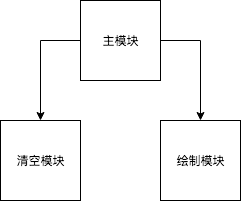
\includegraphics[width=0.3\linewidth]{call.png}
%    \caption{模块关系}
%    \label{fig:call}
%\end{figure}

\section{实验过程}

\subsection{清空}

\par 我的晴空功能只需要通过draw\_button函数即可实现。它画出一个巨大的矩形清空屏幕并放置一个按钮。

\subsection{绘制}
我将touch\_read分为两个部分。touch\_read1是原touch\_read函数,on\_touch\_read\_finish负责连点成线。其使用数组保存多个手指的历史位置。
如果发现点击的位置在按钮内,则触发清空函数。
否则,它将根据触摸点编号,在当前点和上一次的该触摸点之间画一条线。
%\par 绘制模块通过在两个点连线的每一个像素上绘制一定大小和颜色的实心圆来实现绘制连贯、有一定宽度的线的功能。这种实现的主要优点是简单易实现,缺点是进行了大量的重复绘制(两个间隔1px圆存在大量重合的部分)。更好的实现是计算切线,相应地绘制两个半圆和一个矩形。出于时间和难度等原因,未采用这种实现。
%\par 绘制模块总共实现了fb\_draw\_circle和fb\_draw\_thick\_line两个函数,其中fb\_draw\_circle函数负责在指定点绘制指定大小、颜色的实心圆,fb\_draw\_thick\_line负责在两点连线的每一个像素上调用fb\_draw\_circle函数以画线。
%\par fb\_draw\_circle函数在指定正方形区域内遍历每一个点(像素)是否在圆内(即到圆心的距离是否小于等于半径)来决定是否绘制该像素。fb\_draw\_circle的流程如图\ref{fig:drawcirc}所示。
%\begin{figure}[htpb]
%    \centering
%    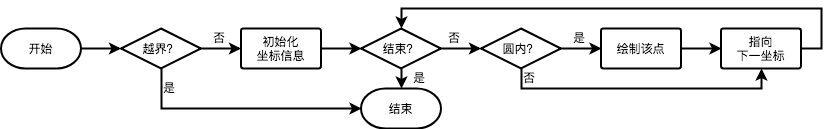
\includegraphics[width=0.8\linewidth]{drawcirc.png}
%    \caption{fb\_draw\_circle流程}
%    \label{fig:drawcirc}
%\end{figure}
%\par fb\_draw\_thick\_line同实验二中的画线函数类似。在最初的实现中,当线过于陡峭时,会出现线不连贯的情况。经过排查是因为最初的实现通过x计算点y,当斜率大于1时,即使是很小的x的变化也会引起y的很大变化。导致两个点距离过大,画出的圆无法连接成线。
%\par 最终实现的fb\_draw\_thick\_line通过检查斜率与1的关系来决定是按照x(斜率小于1)还是y(斜率大于1)来计算每一个点(x, y)。并在该点上调用fb\_draw\_circle函数。fb\_draw\_thick\_line的流程如图\ref{fig:thickline}所示。
%\begin{figure}[htpb]
%    \centering
%    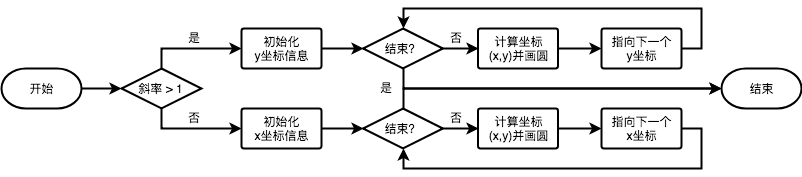
\includegraphics[width=0.8\linewidth]{thickline.png}
%    \caption{fb\_draw\_thick\_line流程}
%    \label{fig:thickline}
%\end{figure}
\subsection{测试}
\par 在测试时,出现了画出的线断断续续的问题,经过长时间排查,最终确定了原因是画线函数的问题。
\par 通过临时修改画线函数后,程序行为恢复正常。

%\subsection{主模块}
%\par 如实验设计所述,主模块的本质是一个无限循环,在循环内部轮询以获取触摸事件。主模块需要保存5个不同触摸点的历史坐标信息以及新读取到的坐标、触摸点信息。主模块对于三种不同的触摸事件,需要作出如下的响应:
%\begin{enumerate}
%    \item TOUCH\_MOVE:主模块需要获取触摸点编号(0-4),并根据编号设置相应的颜色、宽度(用于区分不同的触摸点),并且绘制一条从该触摸点的上一个坐标到当前坐标的直线,并更新该触摸点的历史坐标。
%    \item TOUCH\_PRESS:主模块需要记录该次触摸的坐标以及触摸点信息,并更新该触摸点的历史坐标。
%    \item TOUCH\_RELEASE:主模块需要记录该次释放的坐标即触摸点信息,并和TOUCH\_PRESS中记录的信息进行比对。如果TOUCH\_PRESS和TOUCH\_RELEASE事件的坐标都在清空按钮的坐标范围内,并且是同一种触摸点的话,则证明是按下了清空按钮。需要执行清空操作,并更新该触摸点的历史坐标。
%\end{enumerate}
%\par 主模块的流程如图\ref{fig:main}所示。
%\begin{figure}[htpb]
%    \centering
%    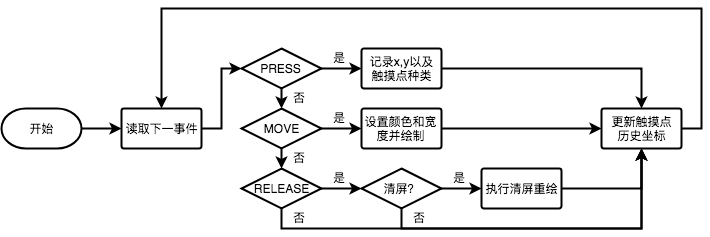
\includegraphics[width=0.8\linewidth]{main.png}
%    \caption{主模块流程}
%    \label{fig:main}
%\end{figure}

\chapter{Linux LED 驱动和控制界面}
\section{实验内容}

\begin{enumerate}
    \item 编写LED驱动:初始化、LED控制函数;
    \item 使用模块方式编译、安装驱动;
    \item 编写测试程序,绘制界面并控制LED驱动;
\end{enumerate}

\section{实验设计}
\par 由于LED的闪烁不能受到画面绘制、手势识别等界面有关的程序的影响,因此需要2个线程或进程共同完成这一任务。为了便于通信以及程序的编写,最终决定采用两个县城完成这一任务。线程间通信的内容为LED灯的闪烁频率或闪烁时间间隔。两个线程之间的关系如图\ref{fig:threadRelation}所示。从图中可以清晰的看到,对于通信内容频率值而言,由于生产者(主线程)只有一个,消费者(控制LED闪烁的线程)也只有一个,因此在这种情况下进行线程间通信不需要加锁。
幸运的是,这个linux上的pthread库可以正常使用。我的多线程由pthread实现。
\begin{figure}[htpb]
    \centering
    
\includegraphics[width=0.6\linewidth]{threadRelation.png}
    \caption{线程之间的关系}
    \label{fig:threadRelation}
\end{figure}

\par 在此实验中,除了背景外其余的控件均是使用函数直接进行绘制。一共包含5个控件:滑槽、滑槽填充、滑块、弹出框、百分比,其形状以及图层如图\ref{fig:stack}所示,图层越高的控件越后绘制。
%\begin{figure}[htpb]
%    \centering
%    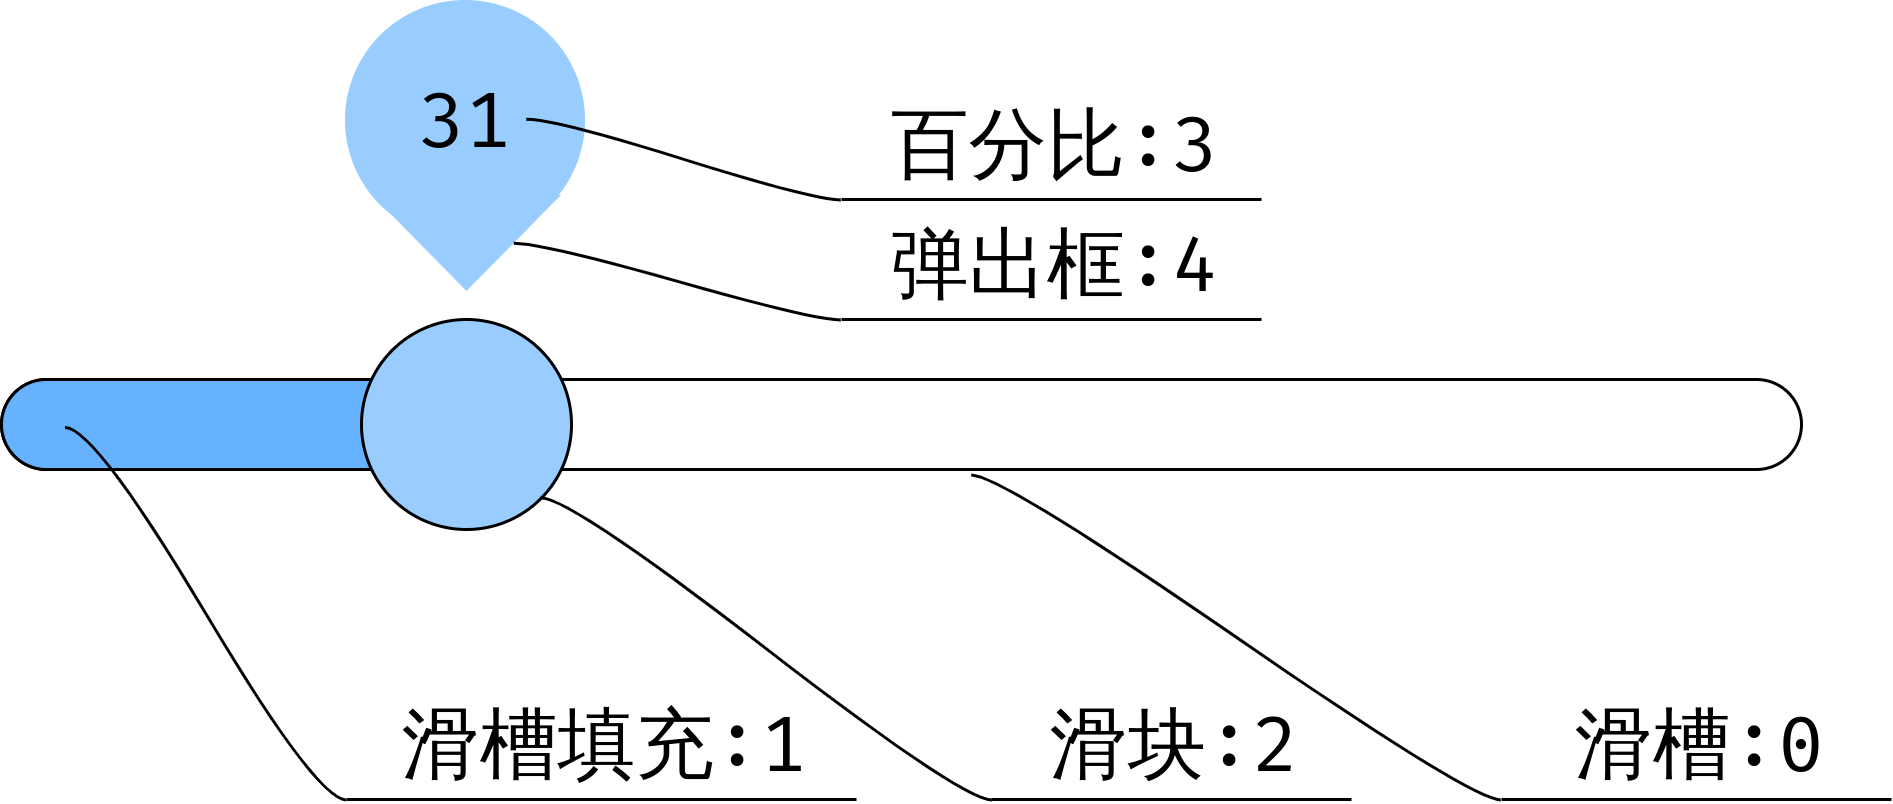
\includegraphics[width=0.4\linewidth]{stack.png}
%    \caption{控件示意图}
%    \label{fig:stack}
%\end{figure}

\par 于是,整个程序被分为了2个模块:界面设计模块以及LED控制模块。对于界面模块而言,其需要运行一个主循环,在循环内不断的判断手势以及手势的位置,然后根据触点的位置判断按钮是否被按下、滑块是否被按下等等。两个线程的流程图如图\ref{fig:flow1}所示。
%\begin{figure}[htpb]
%    \centering
%    
\includegraphics[width=0.9\linewidth]{flow1.png}
%    \caption{两个线程的流程图}
%    \label{fig:flow1}
%\end{figure}

\section{实验过程}
\label{sec:shi_yan_guo_cheng_}
\par 在程序编写完成后,首先使用make编译,然后通过make burn上传开发板并运行。初次运行时发现无论如何拖动滑块LED灯一直为常亮状态。经过仔细的分析源代码后发现这是由于LED闪烁间隔设置得太小造成的,LED闪烁的频率过快导致人眼看起来像是常亮状态。在修改闪烁间隔后,LED能够在人眼能观察到的范围内变化闪烁频率。并在滑块被拖动到两个端点时能够停止闪烁或到达常亮状态。

\addcontentsline{toc}{chapter}{实验心得}
\chapter*{实验心得}
\par 通过这次实验,我对于嵌入式系统有了更为深入的了解,从最开始的系统烧录到最后的上层应用,我对于架构有了更为深入和完整的认知。使我了解了不同的嵌入式平台的不同架构特性,也体会到了linux系统对于在嵌入式平台的优劣。而通过后面对于图形界面的构建,不仅使我了解了平时在其他实验中通过调库构建的图形界面在底层是如何实现的、event loop的具体实现,也使我对于linux底层架构,对于“一切皆文件”这一概念有了更为深入的了解。
\par 这次难度逐级加大的实验对于我最深刻的影响就是对于包括嵌入式linux在内的linux设备文件的了解。实验1~3的内容都能被轻松的移植到x86 linux平台运行,也使我感慨将设备抽象成文件的便利性。对于图形界面的绘制也令我体会到了各种绘图算法的原理,并能够在将来的学习生活中加以应用。

%%%%%%%%%%%%%%%%%%%%%%%%%%%%%%

%\par 这学期的嵌入式实验让我收获颇丰。
%\par 在课余生活中我主要学习的是iOS开发,作为一个开发者接触的一直都是上层封装好的各种接口。但是嵌入式课程以及实验却让我对于iOS的底层ARM有了更多更深入的了解。
%\par 虽然iOS和Android不同,Android采用的是Linux的内核,而iOS采用的是BSD框架下的Darwin内核的修改版,但是其中底层的原理却是相似的。
%\par 通过嵌入式实验,我确实对iOS中手势的识别和传递链、以及图片的完整渲染过程有了更深层的了解。
%\par 本次实验我们小组采用了Git进行协作开发,也增加了我的团队合作能力。
%
%\begin{itemize}
%    \item 实验一中,我主要负责Linux内核的编译以及环境的搭配。我成功的在我的Arch Linux虚拟机中部署了完整的开发环境并进行了测试。不过由于我的笔记本电脑不支持串口通信,最终烧录改在了机房的电脑上,而之后的开发和测试均在我的Arch Linux虚拟机中进行。
%    \item 实验二中,我主要负责矩形和点的绘制,通过这次实验,我了解并学习了Frame Buffer,并且在底层操作Frame Buffer实现了自定义的绘制。虽然现在作为嵌入式开发者(特别是移动开发者),很多时候无需和底层打交道,但是对底层的了解却让我们在关键时候可以分析出性能瓶颈,并进行相应的优化。
%    \item 实验三中,我主要负责PNG图片的绘制和渲染。我主要学习了Alpha通道以及透明度计算的相关知识,也思考了使用矩阵运算优化渲染的思路,最后受限于时间和难度等因素,没有能够实现,还是有一些遗憾的。
%    \item 实验四中,我主要负责了画圆和画线函数。画线是我在实验二中没有负责的部分。通过这次实验,我了解了常见的一些画线算法,也调整了画线算法以解决斜率过大不连贯的问题。最后,我还尝试了解了一些有关抗锯齿的高效画线算法。
%    \item 实验五中,我主要负责UI的绘制。有了前面几次实践的经历,UI的绘制其实非常简单。我也尝试使用了三角形和圆形相连接的方式,实现了稍微复杂的UI(包括复杂形状以及进度的显示和弹出式气泡)。总体上来说,还是很有成就感的。
%\end{itemize}

%%%%%%%%%%%%%%%%%%%%%%%%%%%%%%

%\par 嵌入式开发在上这门课之前,就早已有听说,学校里随处可见的嵌入式开发的实例吸引着我们的注意力,对此仅有模糊的概念。经过对嵌入式系统这门课程的学习以及上机的实验,让我们对嵌入式开发有了很多的认识。
%\par 在嵌入式的理论课上,老师已经为我们讲解了Linux及在嵌入式系统上Linux的应用。
%\par 然而到开始实验的时候才发现很多实验中的内容跟单纯的操作系统差别较大,在第一堂课上基本是依葫芦画瓢照着老师说的一步步做下来,不明白自己的每一步操作的原因和目的,基本的原理也不是很清楚。一旦出错,也不知道从哪儿排错,只能问老师或者助教,但是经过这五次课六次的实验,我们对嵌入式系统有了一个大致清晰的认识和了解,对各个步骤也有了较清晰的认识。
%\par 对于这次的实验仍然有些遗憾的地方,对于嵌入式系统的操作及过程有了较为深刻的认识,但是对于实验过程中用到的程序却基本都不是自己编写的,很多代码只是弄懂了皮毛,没有深刻的理解,当然这些不光是我们编写能力的问题,也有时间等诸多因素。

\appendix
\addcontentsline{toc}{chapter}{实验代码}
{\let\clearpage\relax \chapter*{实验代码}}
\inputCodeSetLanguage{c}
\NewDocumentCommand{\inputCodeFile}{v}{
    \noindent\par #1
    \lstinputlisting{../#1}
}
\inputCodeFile{common/graphic.c}
\inputCodeFile{common/touch.c}
\inputCodeFile{lab1/main.c}
\inputCodeFile{lab2/main.c}
\inputCodeFile{lab3/main.c}
\inputCodeFile{lab4/main.c}
\inputCodeFile{lab5/main.c}

\vfill
{\tiny written by Recolic Keghart <root@recolic.net> (a.k.a. Bensong Liu <bensong@berkeley.edu>), Lu Pan <2951277962@qq.com> \hfill powered by \XeLaTeX .}
\end{document}

